\newpage
\subsection*{Вывод\\}

В данной работе была написана программа для поиска функциональных связей между параметрами. БЫл использован метод наименьших квадратов ввиду его простоты и практичности. Были выведены все формулы для аппроксимации, а также для тестирования приложения был написан генератор случайных зависимостей.

\vspace{0.5cm}

\begin{center}
    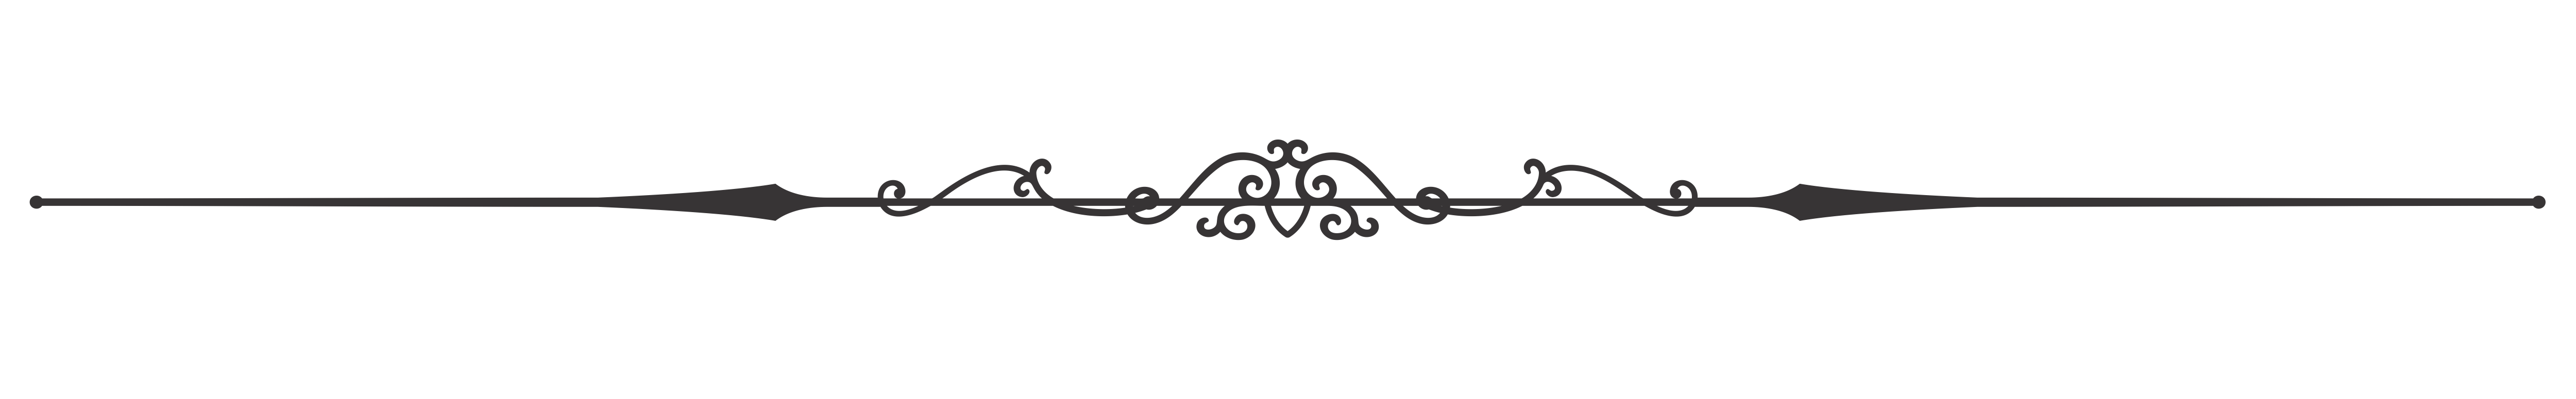
\includegraphics[width=0.75\textwidth]{Screenshots/line.png}
\end{center}